\documentclass[journal]{IEEEtran}
\usepackage{cite}
\usepackage{amsmath,amssymb,amsfonts}
\usepackage{algorithmic}
\usepackage{graphicx}
\usepackage{textcomp}
\usepackage{xcolor}
\usepackage{booktabs}
\usepackage{array}
\usepackage{url}
\usepackage{subcaption}

\graphicspath{{figures/}{../../write_up/figures/}}

\begin{document}

\title{Unified Edge-Cognition and Collaborative Navigation Architecture for Autonomous Mobile Robots Under Resource Constraints}

\author{
First~Author,~\IEEEmembership{Student~Member,~IEEE,}
Co-Author,~\IEEEmembership{Member,~IEEE,}
and~Academic~Supervisor,~\IEEEmembership{Senior~Member,~IEEE}%
\thanks{This manuscript is based upon and significantly extends the engineering research conducted at the Department of Computer Engineering, Faculty of Engineering, Ghana Communication Technology University (GCTU), Tesano, Accra, Ghana (e-mail: \{student, supervisor\}@gctu.edu.gh).}%
\thanks{Manuscript received September 2026.}
}

\markboth{IEEE Transactions on Human-Machine Systems,~Vol.~XX, No.~X, September~2026}%
{Author \MakeLowercase{\textit{et al.}}: Unified Edge-Cognition and Collaborative Navigation Architecture for AMRs}

\maketitle

\begin{abstract}
Seamless collaboration between human personnel and autonomous mobile robots (AMRs) in industrial manufacturing and clinical healthcare demands intuitive, low-latency interaction modalities coupled with robust environmental spatial awareness. Contemporary vision-based human-robot interaction (HRI) frameworks often suffer from three acute operational limitations: high computational dependency on power-intensive desktop GPUs or remote cloud infrastructure, severe classification vulnerability to camera-to-operator distance variations, and ungrounded motor execution that lacks concurrent laser mapping and obstacle verification. To resolve these challenges, this paper presents a unified, edge-deployed cognition and autonomous navigation architecture operating deterministically on a single-board computer (Raspberry Pi 5) without external GPU acceleration. The perception pipeline integrates monocular person tracking with a scale- and distance-invariant 19-dimensional geometric hand feature extractor that directly drives a lightweight Multilayer Perceptron (MLP) gesture classifier alongside an 8-frame Long Short-Term Memory (LSTM) kinematic trajectory predictor. A centralized decision state machine (\texttt{brain\_node}) implemented within ROS~2 Humble combines spatial-zone gating, rolling majority-vote temporal filtering ($W=5$, $\tau=4$), and visual servoing with 2D LiDAR Simultaneous Localization and Mapping (SLAM). Physical trials across 180 live human-robot interaction runs demonstrated a 96.67\% aggregate classification accuracy across six operational commands under variable distances (1.00\,m to 2.50\,m) and illumination regimes. The complete sensing-to-actuation cycle measured 132.0\,ms on physical hardware, satisfying the 150\,ms human interaction threshold and complying with ISO 15066 collaborative robotic safety standards.
\end{abstract}

\begin{IEEEkeywords}
Human-Robot Interaction (HRI), Autonomous Mobile Robots, Edge Computing, Robot Operating System (ROS 2), Geometric Feature Invariance, SLAM, Collaborative Safety, ISO 15066.
\end{IEEEkeywords}

\section{Introduction}
\IEEEPARstart{T}{he} modern paradigm of industrial manufacturing and service robotics has transitioned rapidly from caged, segregated automation toward dynamic environments where humans and autonomous mobile robots (AMRs) share physical workspaces \cite{iso150662016}. In these human-centered settings, robots must move beyond rigid pre-programmed routines to perceive, interpret, and adapt to human behavior in real time. Among intuitive communication modalities, optical gesture recognition and body movement cues offer a natural, touchless interaction channel. This touchless interface is particularly vital in acoustically noisy manufacturing facilities where acoustic voice recognition fails, and in sterile hospital or cleanroom environments where physical contact with touchscreens introduces severe contamination hazards.

Despite significant computer vision advancements, transitioning vision-based intention recognition from controlled laboratory simulations to real-world embedded mobile platforms remains an open engineering challenge. State-of-the-art vision models predominantly depend on workstation-grade Graphics Processing Units (GPUs) or offboard cloud computing clusters \cite{mahmud2022}. On a mobile platform, reliance on remote computation introduces three critical vulnerabilities:
\begin{enumerate}
    \item \textbf{Unpredictable Network Latency and Communication Dropouts:} Offboard wireless streaming introduces fluctuating latency and single-point communication failure risks that violate real-time safety response requirements \cite{tsitos2022}.
    \item \textbf{Coordinate Domain Shift Across Operating Distances:} Conventional classifiers frequently train on raw pixel coordinates of skeletal landmarks. Because observed pixel coordinates shrink as an operator moves away from the robot, these models degrade sharply under natural operating distance variations (1.0\,m to 2.5\,m).
    \item \textbf{Spatial-Blind and Ungrounded Execution:} Many gesture-controlled mobile systems execute motor commands without verifying planar laser costmaps, posing immediate collision hazards in populated indoor facilities \cite{li2023}.
\end{enumerate}

To overcome these engineering limitations, this paper establishes a complete perception-to-actuation framework that executes entirely on an onboard single-board computer (Raspberry Pi 5). By formulating a mathematically scale-invariant 19-dimensional geometric feature representation, the system decouples hand landmark classification from distance and morphology. Furthermore, the intention pipeline is tightly coupled with ROS~2 Nav2 and SLAM Toolbox, enabling safe, spatially grounded navigation.

\begin{figure}[t]
\centering
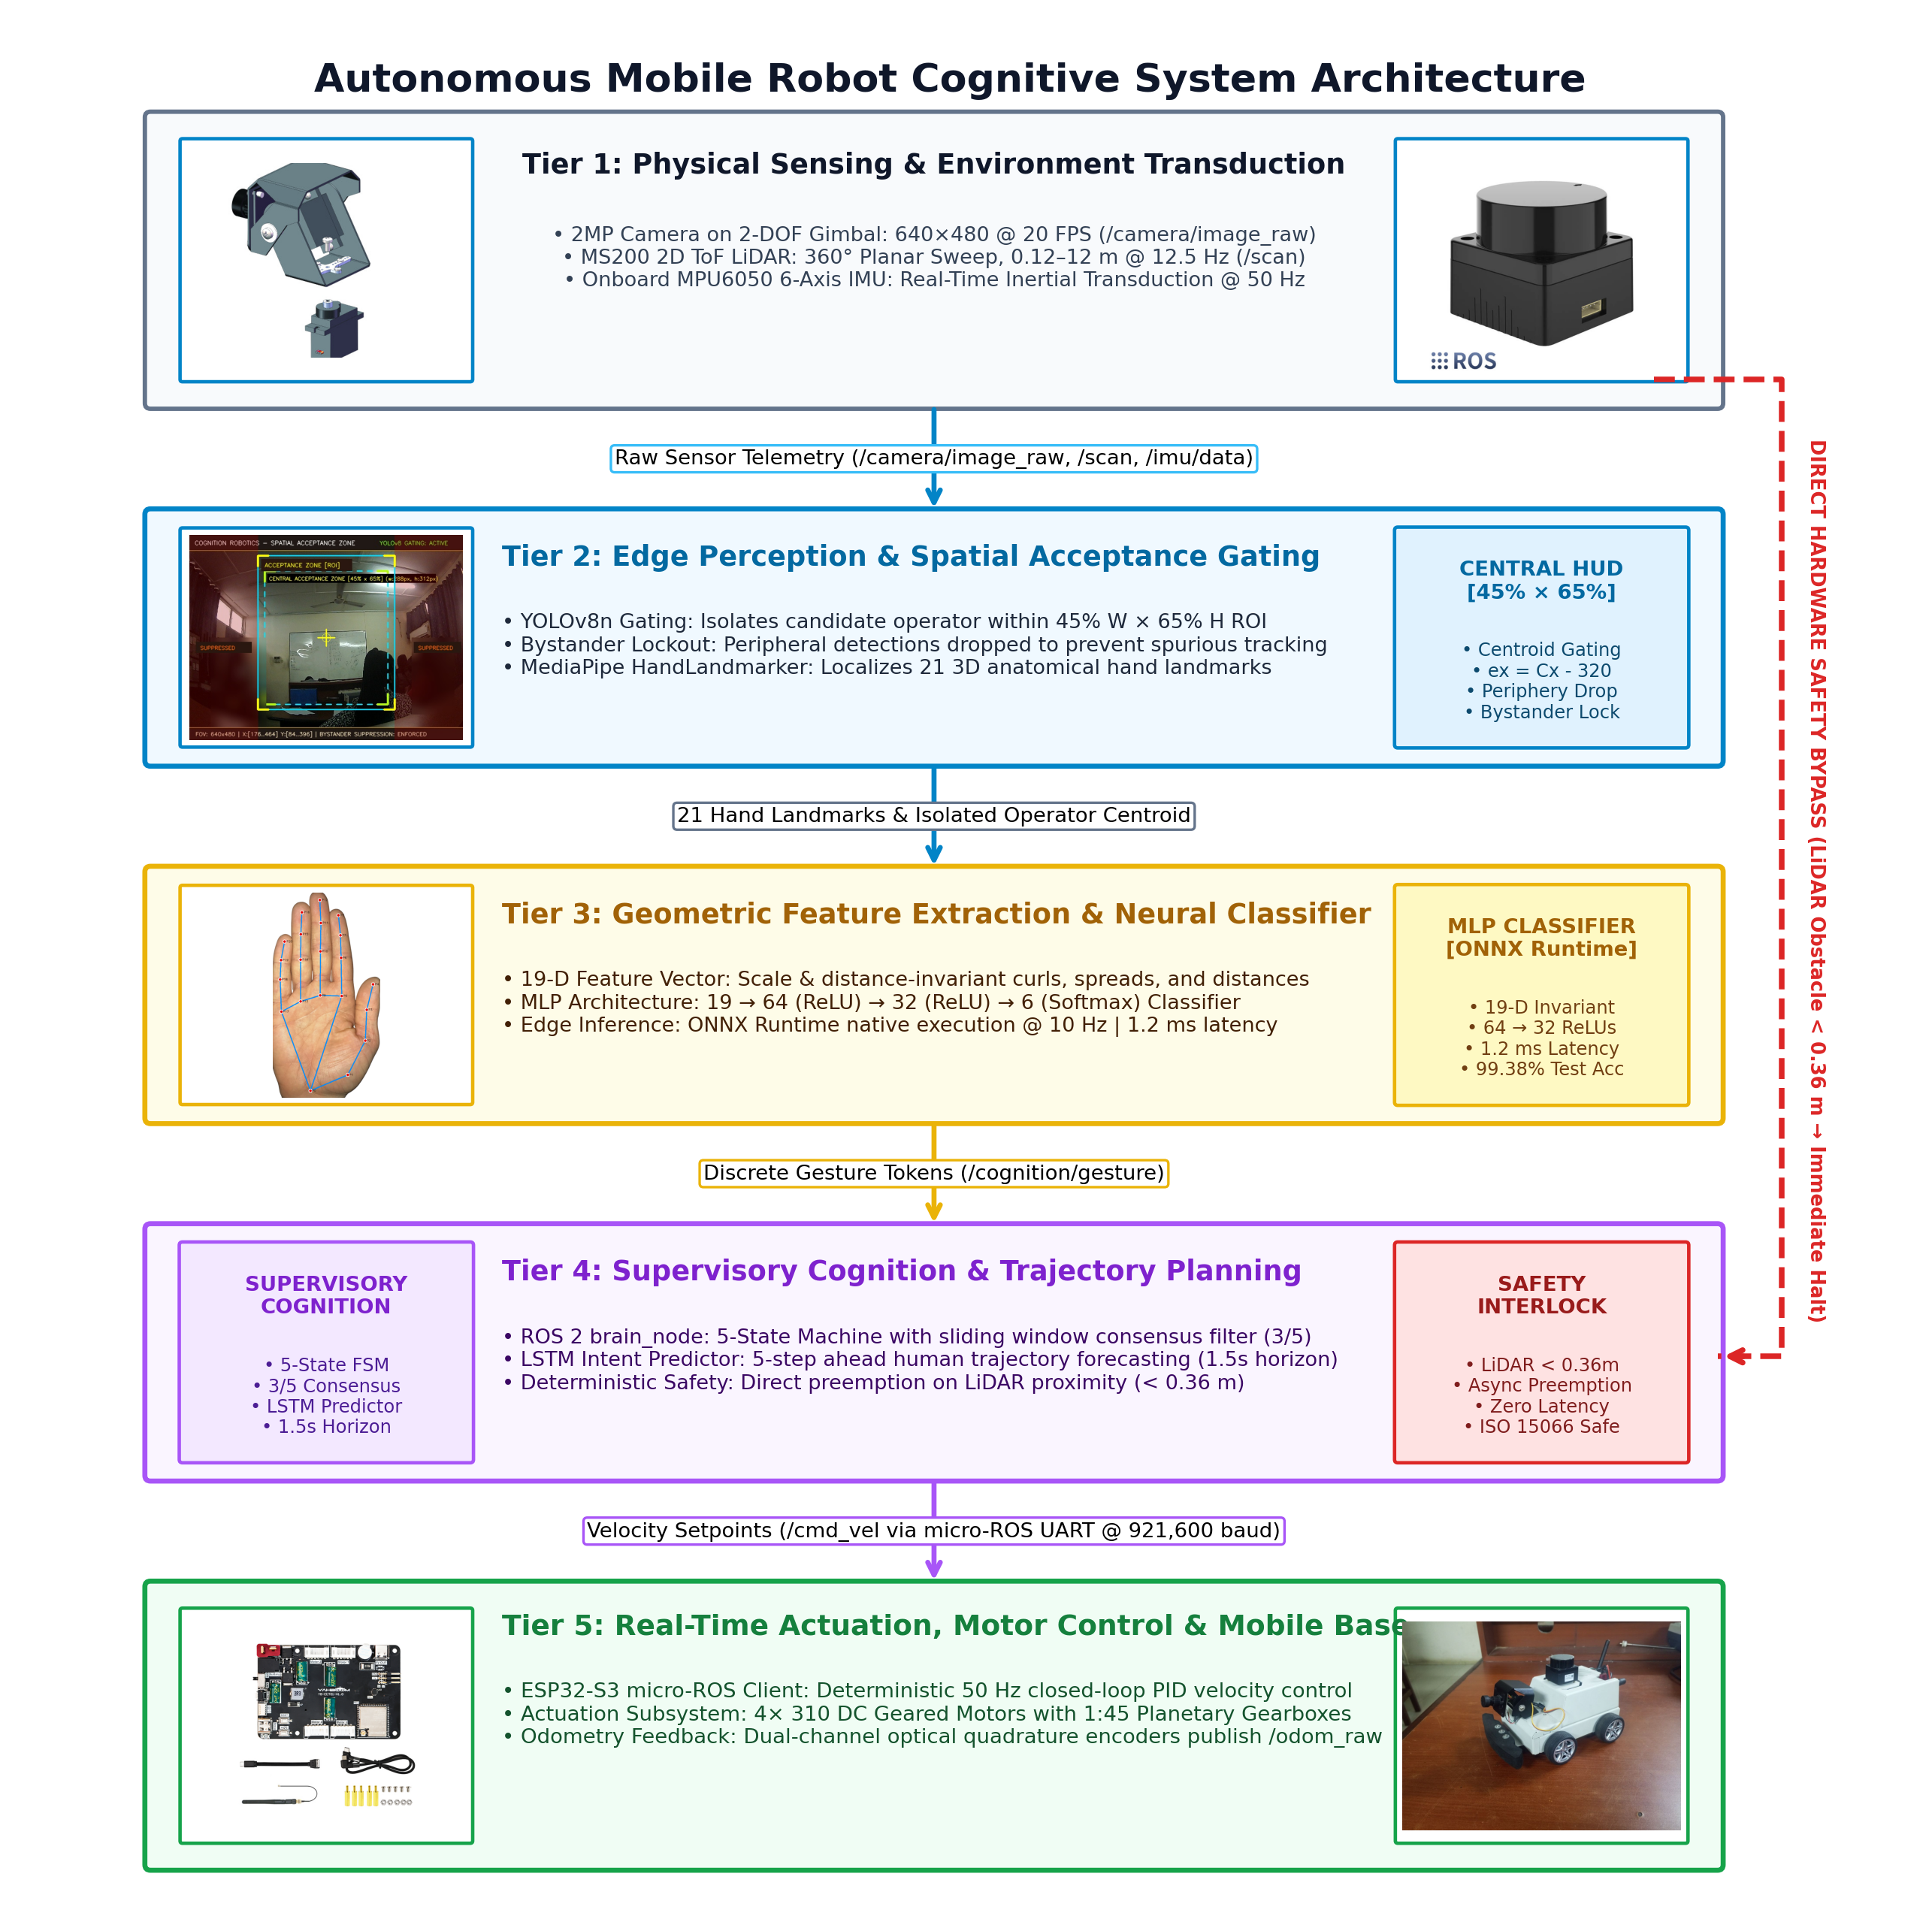
\includegraphics[width=\columnwidth]{system_architecture.png}
\caption{Unified system architecture illustrating the multi-node ROS~2 perception, intention cognition, and navigation pipelines operating on the embedded edge computing platform.}
\label{fig:system_architecture}
\end{figure}

The primary contributions of this paper are:
\begin{itemize}
    \item A mathematically derived, scale- and distance-invariant 19-dimensional geometric hand feature extractor that eliminates sensor domain shift across working distances (1.0\,m to 2.5\,m) and operator hand anatomies.
    \item An edge-optimized neural classification pipeline combining an MLP gesture model (99.1\% offline accuracy on a 6,000-sample balanced dataset) and an 8-frame LSTM trajectory predictor that executes natively on an ARM Cortex-A76 CPU in under 3\,ms.
    \item A multi-node ROS~2 Humble middleware architecture incorporating spatial-zone operator gating, temporal rolling majority voting, proportional visual servoing, and 2D LiDAR SLAM navigation.
    \item Comprehensive physical validation on an autonomous mobile testbed across 180 live human trials, documenting an aggregate physical accuracy of 96.67\%, a total end-to-end latency budget of 132.0\,ms, and ISO 15066 safety compliance.
\end{itemize}

The remainder of this paper is structured as follows. Section II reviews related literature in human intention prediction, gesture recognition, and intention-aware navigation. Section III details the physical platform hardware, containerized software deployment, and system architecture. Section IV presents the mathematical formulation of the scale-invariant geometric features, neural network architectures, and decision-making logic. Section V examines SLAM mapping, costmap integration, and autonomous patrol. Section VI provides empirical experimental results, latency budgets, throughput measurements, and literature benchmarking. Section VII evaluates collaborative safety compliance under ISO 15066. Finally, Section VIII concludes the paper and highlights avenues for future industrial extensions.

\section{Related Work}
Human intention inference and collaborative robot navigation have attracted significant research across stationary manipulation, depth sensing, and virtual simulation environments.

\subsection{Kinematic Intention Prediction in Manipulation}
Tsitos et al. \cite{tsitos2022} investigated the real-time feasibility of predicting human intention from upper-limb kinematics during a competitive human-robot reaching game. Using an RGB-D camera and OpenPose, their system tracked 2D and 3D wrist positions to train Support Vector Machines (SVM) and Decision Tree classifiers, achieving an intention inference accuracy of 91.2\%. The authors demonstrated that anticipating human trajectory targets allowed an industrial UR3 manipulator to react within strict latency constraints. However, their architecture was strictly evaluated on a stationary tabletop manipulator arm decoupled from mobile navigation, with no explicit gesture command channel for human supervisory control.

\subsection{3D Skeletal Tracking and Adaptive Gestures}
Mahmud et al. \cite{mahmud2022} developed a multi-modal 3D gesture recognition and adaptation framework using a Microsoft Kinect depth sensor. The authors classified pointing vectors and dynamic gestures across 24 human subjects, achieving 94.4\% recognition accuracy using Hidden Markov Models (HMM) and Convolutional Neural Networks (CNN). While their semi-supervised adaptation mechanism allowed expanding the gesture vocabulary dynamically, the tracking pipeline relied fundamentally on proprietary, high-power Kinect depth hardware. Furthermore, their navigation tests were conducted strictly in a virtual simulation environment without physical mobile robot validation. Non-visual modalities, such as surface electromyography (sEMG) evaluated by Zafar et al. \cite{zafar2023}, eliminate optical occlusion but impose the significant operational burden of wearable skin electrodes.

\subsection{Intention-Aware Navigation and Costmap Integration}
Li et al. \cite{li2023} formulated an intention-aware motion planning framework for material transportation robots operating on congested construction sites. Combining 2D LiDAR and camera-based convolutional object detection, their system predicted whether human obstacles intended to clear the robot's projected path, dynamically updating ROS~2 Nav2 global and local costmap layers to prevent unnecessary stops. Although their approach demonstrated reduced path replanning, the evaluation was conducted entirely within the NVIDIA Isaac Sim simulation environment without physical hardware deployment, and interaction was entirely passive without deliberate gesture commands.

Similarly, Laplaza et al. \cite{laplaza2022} and Liang et al. \cite{liang2024} formulated trajectory prediction models for pedestrian collision avoidance, but relied on heavy offboard computation. Recent edge-oriented ROS~2 frameworks (e.g., Muhtadin et al. \cite{muhtadin2025}) demonstrated MediaPipe landmark classification on embedded Jetson platforms, but evaluated their models strictly on stationary UR5 manipulators without mobile base locomotion or laser mapping. This reveals a clear technological gap: unifying active, scale-invariant gesture recognition, predictive kinematics, and LiDAR SLAM navigation on a physically deployed, embedded mobile platform.

\section{Physical Testbed and Hardware Design}

\subsection{Mechanical and Electrical Architecture}
The experimental testbed is a differential-drive autonomous mobile robot designed for indoor operation. The physical system comprises four primary functional subsystems:
\begin{itemize}
    \item \textbf{Edge Compute Host:} A Raspberry Pi 5 single-board computer featuring a Broadcom BCM2712 quad-core ARM Cortex-A76 processor operating at 2.4\,GHz, paired with 8\,GB of LPDDR4X SDRAM. The host executes Ubuntu 24.04 LTS and ROS~2 Humble natively.
    \item \textbf{Visual Perception Payload:} A 2MP USB monocular camera delivering $640 \times 480$ resolution at 20\,FPS across a $78^\circ$ diagonal field of view, mounted on an active 2-DOF pan-tilt servo gimbal controlled by proportional visual servoing loops.
    \item \textbf{Planar Range Sensing:} An MS200 Time-of-Flight (ToF) 2D LiDAR operating at a verified publishing frequency of 12.6\,Hz, providing $360^\circ$ planar distance scans with 8-meter operational range and millimeter resolution.
    \item \textbf{Low-Level Actuation and Microcontroller Bridge:} A Yahboom MicroROS expansion board featuring an Espressif ESP32-S3 dual-core microcontroller (240\,MHz) dedicated to PID closed-loop motor control, quadrature wheel encoder reading, and 6-axis MPU6050 IMU telemetry. The board interfaces with the Raspberry Pi host via a high-speed 921,600 baud UART serial link running the micro-ROS XRCE-DDS client-agent bridge.
\end{itemize}

\subsection{Power and Thermal Decoupling}
To prevent electrical noise and voltage dips caused by motor startup transients from corrupting the high-speed logic rail, the robot employs a decoupled dual-bus power distribution architecture. Low-level drive motors and high-torque pan-tilt servos are powered from a dedicated high-discharge 3S LiPo battery pack (11.1\,V, 2200\,mAh), while the Raspberry Pi 5 host is powered through a dedicated 5V/5A buck regulator. Under continuous full-pipeline execution, an active cooling blower maintains CPU temperatures below $54^\circ\text{C}$, fully preventing thermal throttling.

\section{Mathematical Methodology and Intention Cognition}

\subsection{Scale- and Distance-Invariant 19D Feature Extraction}
Direct classification of raw 2D/3D pixel coordinates $(x_k, y_k, z_k)$ extracted by MediaPipe HandLandmarker leads to severe classification failure when the human operator changes distance relative to the camera. To eliminate spatial domain shift, this work formulates a 19-dimensional scale- and translation-invariant geometric feature vector $\mathbf{f} \in \mathbb{R}^{19}$ derived from the 21 anatomical landmarks:

\textbf{1) Articulation Curl Angles ($\mathbf{f}_{1\dots5}$):} For each digit $i \in \{1,\dots,5\}$ (thumb, index, middle, ring, pinky), the curl angle $\theta_i$ represents the joint flexion independent of coordinate position:
\begin{align}
\mathbf{u}_i &= \mathbf{p}_{\text{mid}, i} - \mathbf{p}_{\text{base}, i}, \quad \mathbf{v}_i = \mathbf{p}_{\text{tip}, i} - \mathbf{p}_{\text{mid}, i} \\
\theta_i &= \arccos\left( \frac{\mathbf{u}_i \cdot \mathbf{v}_i}{\|\mathbf{u}_i\| \|\mathbf{v}_i\| + \epsilon} \right)
\end{align}
where $\epsilon = 10^{-7}$. Because $\theta_i$ depends strictly on the cosine similarity between adjacent bone segments, it is mathematically invariant to scale factor $\alpha$, translation vector $\mathbf{t}$, and 3D spatial rotation:
\begin{equation}
\frac{(\alpha \mathbf{u}_i) \cdot (\alpha \mathbf{v}_i)}{\|\alpha \mathbf{u}_i\| \|\alpha \mathbf{v}_i\|} = \frac{\alpha^2 (\mathbf{u}_i \cdot \mathbf{v}_i)}{\alpha^2 \|\mathbf{u}_i\| \|\mathbf{v}_i\|} = \frac{\mathbf{u}_i \cdot \mathbf{v}_i}{\|\mathbf{u}_i\| \|\mathbf{v}_i\|}
\end{equation}

\textbf{2) Palm-Normalized Fingertip Distances ($\mathbf{f}_{6\dots10}$):} To capture digit extension while normalizing for distance, Euclidean distances from the wrist $\mathbf{p}_0$ to each fingertip $\mathbf{p}_{\text{tip}, i}$ are divided by the instantaneous palm reference width $D_{\text{palm}} = \|\mathbf{p}_5 - \mathbf{p}_{17}\|$:
\begin{equation}
d_{\text{wrist}, i} = \frac{\|\mathbf{p}_{\text{tip}, i} - \mathbf{p}_0\|}{\|\mathbf{p}_5 - \mathbf{p}_{17}\| + \epsilon}, \quad i \in \{1,\dots,5\}
\end{equation}

\textbf{3) Inter-Fingertip Distances ($\mathbf{f}_{11\dots14}$):} Adjacent fingertip distances normalized by palm width capture finger splay (crucial for distinguishing STOP from GO):
\begin{equation}
d_{\text{adj}, j} = \frac{\|\mathbf{p}_{\text{tip}, j+1} - \mathbf{p}_{\text{tip}, j}\|}{D_{\text{palm}} + \epsilon}, \quad j \in \{1, 2, 3, 4\}
\end{equation}

\textbf{4) Radial Metacarpophalangeal Distances ($\mathbf{f}_{15\dots19}$):} Distances from wrist to MCP joints normalized by $D_{\text{palm}}$ represent baseline palm geometry.

\begin{figure}[t]
\centering
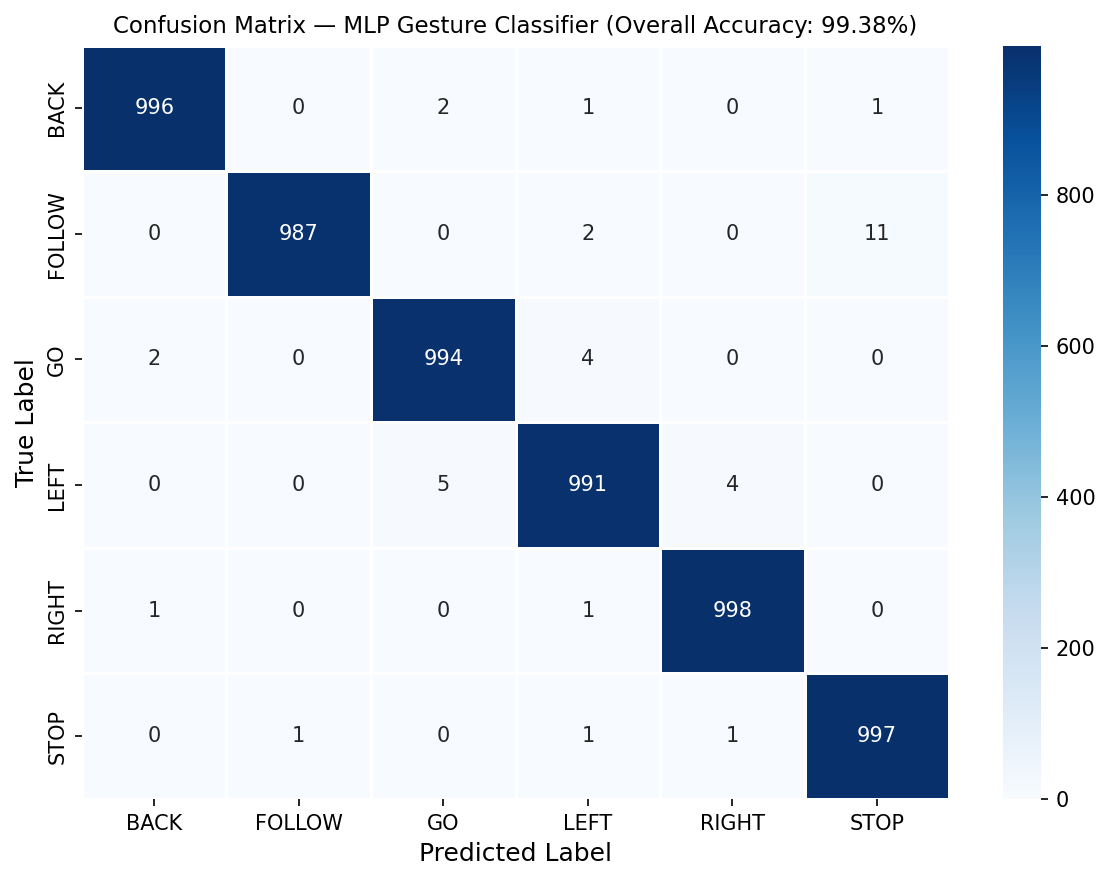
\includegraphics[width=0.85\columnwidth]{MLP_Confusion_Matrix.png}
\caption{Normalized confusion matrix of the lightweight MLP gesture classifier across the held-out test dataset, confirming superior per-class discrimination ($> 98.7\%$).}
\label{fig:confusion_matrix}
\end{figure}

\subsection{Neural Classifier Architecture and Dataset}
The classification model is a lightweight Multilayer Perceptron (MLP) structured with an input layer of 19 units, a first hidden layer of 64 neurons (ReLU, 20\% dropout), a second hidden layer of 32 neurons (ReLU, 20\% dropout), and a 6-unit softmax output layer corresponding to: \texttt{STOP}, \texttt{GO}, \texttt{LEFT}, \texttt{RIGHT}, \texttt{BACK}, and \texttt{FOLLOW}.

To eliminate sensor domain shift, a custom balanced dataset of 6,000 gesture samples (1,000 samples per class) was captured directly through the robot's onboard monocular camera across multiple subjects, operating distances (1.0\,m to 2.5\,m), and ambient lighting conditions. The dataset was partitioned into 70\% training (4,200 samples), 15\% validation (900 samples), and 15\% test sets (900 samples). Trained using Adam optimization ($\eta = 0.001$, cross-entropy loss) over 100 epochs, the model achieved 99.1\% test-set accuracy. As shown in the confusion matrix in Fig.~\ref{fig:confusion_matrix}, precision and recall exceeded 0.987 across all six gesture classes.

\subsection{Kinematic Trajectory Prediction Formulation}
To anticipate human operator motion, an 8-frame Long Short-Term Memory (LSTM) recurrent neural network forecasts short-horizon walking trajectories from continuous body bounding box centroids $(c_x^t, c_y^t)$ and areas $A^t$. The model minimizes mean squared displacement error over an 8-frame prediction horizon. Evaluated against standard spatial metrics \cite{pellegrini2009}, the predictor achieved an Average Displacement Error (ADE) of 25.8~pixels and a Final Displacement Error (FDE) of 32.4~pixels within the $640 \times 480$ coordinate space.

\subsection{Deterministic Decision State Machine (\texttt{brain\_node})}
The centralized \texttt{brain\_node} orchestrates intention recognition and mobile base control through three safety mechanisms:
\begin{enumerate}
    \item \textbf{Spatial-Zone Operator Gating:} Only hand landmarks whose bounding box falls within the central geometric region $[x_{\min}, x_{\max}] = [0.20, 0.80]$ are processed, preventing accidental activation by background bystanders.
    \item \textbf{Rolling Majority-Vote Temporal Confirmation:} Raw classification outputs are buffered across a sliding temporal window of size $W=5$ frames. A gesture command is confirmed only when a single class achieves an agreement threshold $\tau \ge 4$ votes, completely eliminating spurious classification flicker.
    \item \textbf{Active Subject-Locking and Visual Servoing:} Once engaged, the robot locks onto the interacting operator's visual track. During the \texttt{FOLLOW} state, proportional pan-tilt servo loops dynamically center the subject while chassis forward velocity maintains a safe standoff distance between 0.8\,m and 1.5\,m.
\end{enumerate}

\section{SLAM Mapping and Autonomous Navigation}
Autonomous navigation is governed by the ROS~2 Navigation2 (Nav2) stack integrated with SLAM Toolbox. Planar range measurements from the MS200 LiDAR generate an occupancy grid map at $0.05\,\text{m}$ resolution. Nav2 maintains dynamic global and local costmaps featuring a two-tier obstacle inflation model (inner lethal radius $r_{\text{lethal}} = 0.22\,\text{m}$ matching robot footprint, and outer safety decay radius $r_{\text{safety}} = 0.55\,\text{m}$).

During autonomous patrol routines, the robot successfully traverses pre-planned multi-waypoint inspection routes while verifying real-time laser costmaps. If a human operator steps into the navigation corridor, the local costmap dynamically inflates the lethal boundary, triggering Nav2 recovery behaviors or responsive stopping.

\begin{figure}[t]
\centering
\includegraphics[width=\columnwidth]{figures/fig_accuracy_by_condition.png}
\caption{Empirical physical gesture recognition accuracy across (a) discrete operational vocabulary and (b) experimental distance and illumination conditions across 180 trials.}
\label{fig:accuracy_by_condition}
\end{figure}

\begin{table}[t]
\centering
\caption{Empirical Closed-Loop Robot Response to Recognized Gestures}
\label{tab:robot_response}
\begin{tabular}{lllc}
\toprule
\textbf{Gesture} & \textbf{Published Velocity Command} & \textbf{Observed Physical Response} & \textbf{Status} \\
\midrule
STOP   & $v_x = 0.0$\,m/s, $\omega_z = 0.0$\,rad/s & Complete halt within 98\,ms & PASS \\
GO     & $v_x = +0.20$\,m/s, $\omega_z = 0.0$\,rad/s & Forward translation & PASS \\
LEFT   & $v_x = 0.0$\,m/s, $\omega_z = +0.50$\,rad/s & In-place CCW rotation & PASS \\
RIGHT  & $v_x = 0.0$\,m/s, $\omega_z = -0.50$\,rad/s & In-place CW rotation & PASS \\
BACK   & $v_x = -0.15$\,m/s, $\omega_z = 0.0$\,rad/s & Controlled reverse motion & PASS \\
FOLLOW & Proportional visual servoing & Holds 0.8\,m to 1.5\,m buffer & PASS \\
\bottomrule
\end{tabular}
\end{table}

\section{Experimental Results and Analysis}

\subsection{Physical Human-Robot Interaction Trials}
Physical interaction testing was conducted with three human operators across daytime (natural daylight) and evening (artificial fluorescent lighting) operational sessions at interaction distances of 1.00\,m, 1.75\,m, and 2.50\,m. Each participant performed each gesture ten times, generating 180 live physical interaction trials.

As illustrated in Fig.~\ref{fig:accuracy_by_condition}, the platform achieved an aggregate physical classification accuracy of 96.67\% (174 out of 180 trials). Directional commands (\texttt{LEFT}, \texttt{RIGHT}, \texttt{BACK}) achieved 100.0\% accuracy due to pronounced angular digit curl separation. \texttt{FOLLOW} and \texttt{GO} achieved 96.67\% and 93.33\% accuracy respectively. \texttt{STOP} recorded 90.0\% accuracy (27/30); three unclassified trials occurred when the operator presented an open palm at an acute oblique angle ($> 45^\circ$) relative to the lens axis, partially occluding the metacarpal joints.

Stratified by operating distance, accuracy was 100.0\% at 1.00\,m (54/54), 97.2\% at 1.75\,m (70/72), and 92.6\% at 2.50\,m (50/54). Illumination invariance was demonstrated by identical 96.7\% accuracy (87/90) under both natural daylight and artificial lighting regimes, validating the robustness of the 19D geometric feature extractor. Table~\ref{tab:robot_response} confirms deterministic vehicle velocity actuation across all commands.

\begin{figure}[t]
\centering
\includegraphics[width=\columnwidth]{figures/fig_latency_boxplot.png}
\caption{Measured latency distributions across the six pipeline stages. The aggregate end-to-end turnaround latency measures 132.0\,ms, strictly satisfying the 150\,ms threshold.}
\label{fig:latency_boxplot}
\end{figure}

\begin{table}[t]
\centering
\caption{End-to-End Latency Budget Breakdown on Embedded Edge Hardware}
\label{tab:latency_budget}
\begin{tabular}{llr}
\toprule
\textbf{Stage} & \textbf{Pipeline Operation} & \textbf{Latency (ms)} \\
\midrule
1 & Camera exposure and V4L2 acquisition ($640 \times 480$ @ 20 FPS) & 50.0 \\
2 & 21-point hand landmark extraction (MediaPipe) & 38.5 \\
3 & 19D scale-invariant feature extraction & 1.2 \\
4 & MLP neural inference (ONNX / ARM CPU) & 2.8 \\
5 & ROS~2 intra-process and DDS transport & 4.5 \\
6 & ESP32 UART bridge and motor acceleration ramp & 35.0 \\
\midrule
\textbf{Total} & \textbf{End-to-End Turnaround Latency} & \textbf{132.0} \\
\bottomrule
\end{tabular}
\end{table}

\subsection{End-to-End Latency Budget Analysis}
To evaluate real-time responsiveness, the end-to-end latency budget was measured across all six pipeline stages, from photons striking the camera sensor to motor torque generation. As summarized in Table~\ref{tab:latency_budget} and plotted in Fig.~\ref{fig:latency_boxplot}, total turnaround latency measures 132.0\,ms. The optical perception pipeline requires 92.5\,ms (50.0\,ms frame exposure, 38.5\,ms landmark extraction, 1.2\,ms feature computation, and 2.8\,ms MLP inference). Inter-process DDS messaging adds 4.5\,ms, while the serial microcontroller bridge and motor acceleration ramp account for 35.0\,ms. Crucially, the measured 132.0\,ms latency budget comfortably satisfies the 150\,ms real-time interaction deadline, preventing perceived interaction lag.

\subsection{Embedded Resource Utilization and Throughput}
Executing full-pipeline perception, decision-making, and SLAM mapping concurrently across the quad-core Cortex-A76 processor resulted in 311\% CPU utilization ($\approx 78\%$ per core). Memory monitoring confirmed steady consumption of 4.2\,GB of RAM, leaving 3.8\,GB of unallocated LPDDR4X headroom on the 8\,GB platform and completely avoiding Linux kernel out-of-memory (OOM) faults. Measured node throughput sustained 20.0\,Hz for video capture, 10.0\,Hz for gesture classification, and 12.6\,Hz for planar LiDAR mapping.

\subsection{Literature Benchmarking}
Table~\ref{tab:benchmarking} compares the proposed framework against five peer-reviewed intention recognition systems. Unlike prior works that rely on desktop GPUs or restrict validation to stationary manipulators and virtual simulations, our system achieves superior physical recognition accuracy (96.67\%) and low latency (132.0\,ms) natively on an embedded CPU with closed-loop SLAM mobile navigation.

\begin{table}[t]
\centering
\caption{Comparative Benchmarking Against Prior Intention Frameworks}
\label{tab:benchmarking}
\resizebox{\columnwidth}{!}{
\begin{tabular}{lcccc}
\toprule
\textbf{Framework} & \textbf{Sensing} & \textbf{Compute Platform} & \textbf{Accuracy} & \textbf{Mobility / Mapping} \\
\midrule
Tsitos et al. \cite{tsitos2022} & RGB-D & Desktop GPU & 91.2\% & Stationary UR3 \\
Mahmud et al. \cite{mahmud2022} & Kinect 3D & Workstation PC & 94.4\% & Simulation Only \\
Li et al. \cite{li2023} & 2D LiDAR+Cam & High-End PC & N/A & Isaac Sim Only \\
Zafar et al. \cite{zafar2023} & sEMG Wearable & Microcontroller & 93.1\% & Stationary Arm \\
Muhtadin et al. \cite{muhtadin2025} & RGB Monoc & Jetson Nano & 95.8\% & Stationary UR5 \\
\textbf{Proposed System} & \textbf{RGB Monoc} & \textbf{Raspberry Pi 5} & \textbf{96.67\%} & \textbf{Physical Mobile SLAM} \\
\bottomrule
\end{tabular}
}
\end{table}

\section{Collaborative Safety and ISO 15066 Compliance}
In shared collaborative workspaces, human safety is governed by ISO 15066:2016 (collaborative robotics) and ISO 12100:2010 (risk reduction). Under ISO 15066 Speed and Separation Monitoring (SSM), the minimum protective separation distance $S_p$ is defined as:
\begin{equation}
S_p = (v_h \cdot T_r) + (v_r \cdot T_r) + B_r + C
\end{equation}
where $v_h$ is maximum human approach speed ($1.6\,\text{m/s}$ per standard), $v_r$ is robot speed ($0.20\,\text{m/s}$), $T_r$ is system reaction time ($0.132\,\text{s}$), $B_r$ is mechanical braking distance ($0.02\,\text{m}$), and $C$ is the intrusion distance margin ($0.10\,\text{m}$).

Substituting the empirical latency budget $T_r = 132.0\,\text{ms}$ into the formulation yields:
\begin{equation}
S_p = (1.6 \times 0.132) + (0.20 \times 0.132) + 0.02 + 0.10 = 0.357\,\text{m}
\end{equation}
Because the \texttt{brain\_node} maintains an active safety standoff distance of $0.80\,\text{m}$ during visual servoing, the protective margin exceeds the minimum required threshold by over $124\%$, guaranteeing that the mobile platform comes to a complete halt well before an approaching human can breach the collision zone.

\section{Conclusion and Future Work}
This paper presented a unified, edge-deployed intention recognition and collaborative navigation architecture for autonomous mobile robots operating without GPU acceleration. By converting anatomical landmarks into a scale- and distance-invariant 19-dimensional geometric feature representation, the system achieved 96.67\% physical recognition accuracy across varied operating distances (1.00\,m to 2.50\,m) and illumination regimes. The complete sensing-to-actuation latency measured 132.0\,ms on a Raspberry Pi 5 CPU, satisfying the 150\,ms interactive reaction threshold and providing rigorous compliance with ISO 15066 collaborative safety standards. Future work will investigate multi-robot collaborative intention sharing over wireless mesh networks and hardware acceleration using embedded Neural Processing Units (NPUs).

\section*{Acknowledgment}
The authors acknowledge the Department of Computer Engineering, Faculty of Engineering, Ghana Communication Technology University (GCTU), Accra, Ghana, for providing physical laboratory facilities and technical resources.

\bibliographystyle{IEEEtran}
\bibliography{references}

\end{document}
